%!TEX program = xelatex
\documentclass[10pt, compress, handout]{beamer}
\usepackage[titleprogressbar]{../../cls/beamerthemem}

\setbeamertemplate{caption}[numbered]
\setbeamertemplate{theorems}[numbered]
\newcounter{example}
\resetcounteronoverlays{example}
\newtheorem{crl}{Corollary}[theorem]
\newtheorem{eg}[example]{Example}
\newtheorem*{solution*}{Solution}

\usepackage{booktabs}
\usepackage[scale=2]{ccicons}
\usepackage{minted}

\usepackage{cleveref}
\crefname{example}{Example}{Examples}

\usepgfplotslibrary{dateplot}

\usemintedstyle{trac}

\usepackage{algorithm}
\usepackage[noend]{algpseudocode}
\resetcounteronoverlays{algorithm}

\usepackage{version}
% \excludeversion{proof}
% \excludeversion{solution*}

\usepackage{mathtools}
\usepackage{multicol}
\usepackage{qtree}

\usepackage{tikz}

\makeatletter
\def\old@comma{,}
\catcode`\,=13
\def,{%
    \ifmmode%
    \old@comma\discretionary{}{}{}%
    \else%
    \old@comma%
    \fi%
}
\makeatother

\title{CSCI 3190 Tutorial of Week 12}
\subtitle{Tree}
\author{LI Haocheng}
\institute{Department of Computer Science and Engineering}

\begin{document}

\maketitle

\begin{frame}[fragile]
\frametitle{Complexity}
\onslide<1->\begin{eg}
    Show the following:\begin{enumerate}[(a)]
        \item $3n^2 + 5n + 10 = O(n^2)$
    \end{enumerate}
\end{eg}
\onslide<2>\begin{proof}
    \begin{enumerate}[(a)]
        \item \begin{description}
            \item[Method 1] $\exists c = 4, \exists N = 6$, such that $\forall n > N, 3n^2 + 5n + 10 < 4n^2$.
            \item[Method 2] Since $3 + \frac{5}{n} + \frac{10}{n^2} = O(1)$ and $n^2 = O(n^2)$, $3n^2 + 5n + 10 = O(n^2)$.
        \end{description}
    \end{enumerate}
\end{proof}
\end{frame}

\begin{frame}[fragile]
\frametitle{Terminology}
\begin{columns}
    \begin{column}{.6\linewidth}
        \onslide<1->\begin{eg}
            In the rooted tree $T$ (with root $a$) shown in Figure \ref{f-11-1-5}, find the parent of $c$, the children of $g$, the
            siblings of $h$, all ancestors of $e$, all descendants of $b$, all internal vertices, and all leaves. What
            is the subtree rooted at $g$?
        \end{eg}
        \onslide<2>\begin{solution*}
            The parent of $c$ is $b$. The children of $g$ are $h$, $i$, and $j$. The siblings of $h$ are $i$ and $j$. The ancestors of $e$ are $c$, $b$, and $a$. The descendants of $b$ are $c$, $d$, and $e$. The internal vertices are $a$, $b$, $c$, $g$, $h$, and $j$. The leaves are $d$, $e$, $f$, $i$, $k$, $l$, and $m$.
        \end{solution*}
    \end{column}
    \onslide<1->\begin{column}{.4\linewidth}
        \begin{figure}
            \centering
            $\Tree [.a [.b [.c d e ] ] f [.g [.h k ] i [.j l m ]]]$
            \caption{A Rooted Tree $T$}
            \label{f-11-1-5}
        \end{figure}
    \end{column}
\end{columns}
\end{frame}

\begin{frame}[fragile]
\frametitle{Newark}
\onslide<1->\begin{columns}
    \begin{column}{.5\linewidth}
        \begin{eg}
            Find a shortest route in distance between Newark and
            Camden, and between Newark and Cape May, using
            these roads.
        \end{eg}
    \end{column}
    \begin{column}{.5\linewidth}
        \begin{figure}
            \centering
            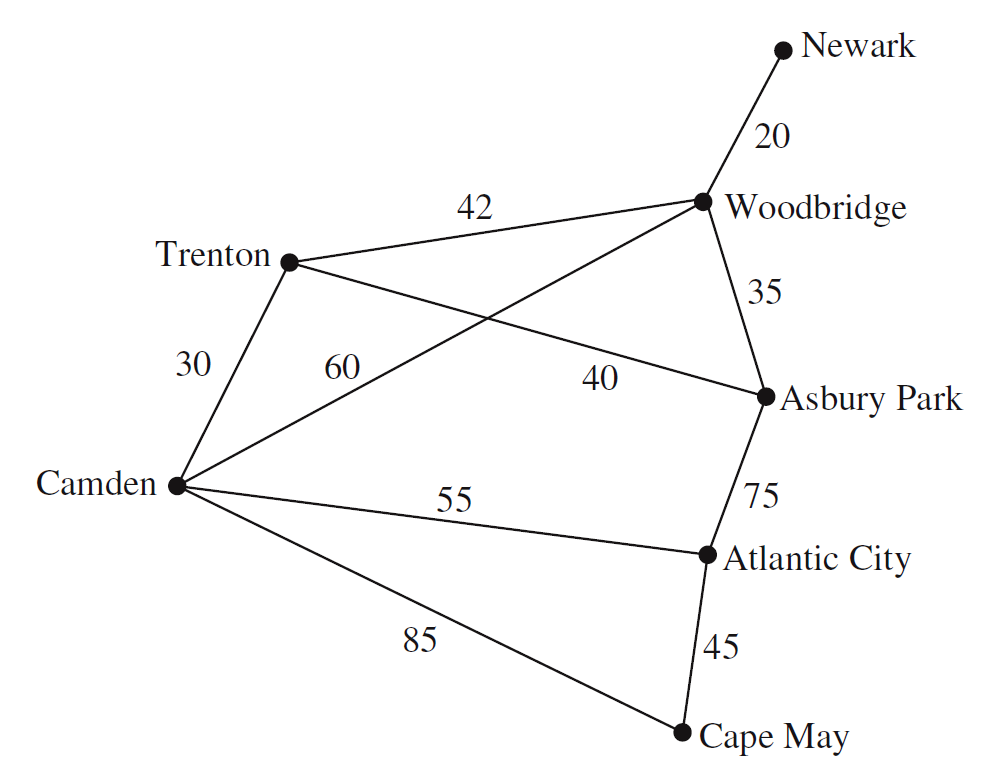
\includegraphics[width=\linewidth]{f-10-6-e-17-a}
        \end{figure}
    \end{column}
\end{columns}
\onslide<2>\begin{solution*}
    \begin{description}
        \item[Camden] 80
        \item[Cape May] 165
    \end{description}
\end{solution*}
\end{frame}

\plain{Questions?}

\end{document}
